%stats cheat sheet
\documentclass[12pt]{article}
\usepackage{amsmath}
\usepackage{geometry}                % See geometry.pdf to learn the layout options. There are lots.
\geometry{letterpaper}                   % ... or a4paper or a5paper or ... 
%\geometry{landscape}                % Activate for for rotated page geometry
\usepackage[parfill]{parskip}    % Activate to begin paragraphs with an empty line rather than an indent
\usepackage{graphicx}
\usepackage{amssymb}
\usepackage{epstopdf}
\DeclareGraphicsRule{.tif}{png}{.png}{`convert #1 `dirname #1`/`basename #1 .tif`.png}

\usepackage{mathtools}

\usepackage{multirow}

\usepackage{tikz}
\def\layersep{2.5cm}

\usepackage[]{algorithm2e}

\title{Stats Summary}
%\author{Aviv}
\date{}                                           % Activate to display a given date or no date

\begin{document}
\maketitle
%\section{}
%\subsection{}


\newcommand{\y}{\mathbf{y}}
\newcommand{\X}{\mathrm{\mathbf{X}}}
\newcommand{\bta}{{\pmb{\beta} } }
\newcommand{\PP}{{\mathrm{\mathbf{P} } } }





\section{Linear Regression}

\paragraph{Linear Regression:} 
A linear combination of $n$ weights ($\theta$) and features ($x$) defining a relationship (hypothesis) between $m$ sets of observations and predictions:
\[
y = \theta_0 + \theta_1 x_1 + \theta_2 x_2 = h_\theta(x)
\]
Note that here $x$ is a single column vector representing one data row. Using the convention that the intercept term $x_0 = 1$ (\textbf{do not forget to add!}), then:

\[
h(x) = \sum_{i=0}^n \theta_i x_i = {\theta}^t  x
\]



To obtain the $\theta_i$ we define a (vector valued) cost function over all $m$ samples:
\begin{align*}
J(\theta) 
=& \frac{1}{2m}\sum_{i=1}^{m} (y^{(i)} - \hat y^{(i)} )^2\\
=& \frac{1}{2m}\sum_{i=1}^{m} (y^{(i)} - h_\theta(x^{(i)}))^2\\
%=& \frac{1}{2m}\sum_{i=1}^{m} 
%\left(y^{(i)} - \sum_{j=0}^{n}\theta_j x_j^{(i)} \right)^2\\
=& \frac{1}{2m}\sum_{i=1}^{m} (y^{(i)} - \theta^t x^{(i)})^2
\end{align*}

Or, fully vectorized, where $X$ is a $m \times n$ matrix:
\[
J(\theta) = \frac{1}{2m} (y - X\theta)^T \, (y - X\theta)
\]

Want to choose $\theta$ as to minimize $J(\theta)$. One option is to use a gradient descent algorithm, which starts with an initial guess and repeatedly performs the update:
\[
\theta_{k} \coloneqq \theta_k - \alpha \frac{\partial}{\partial \theta_k} J(\theta)
\]

The update is simultaneously performed on all values of $k = 1:n$ (we have m rows/observations, and n features).

What is $\frac{\partial}{\partial \theta_k} J(\theta)$?

\begin{align*}
\frac{\partial}{\partial \theta_k} J(\theta)
&= \frac{\partial}{\partial \theta_k} \, \frac{1}{2}\left( h_\theta(x) - y\right)^2
\\
&= 2 \cdot \frac{1}{2}\left( h_\theta(x) - y\right) \cdot\frac{\partial}{\partial \theta_k} \left( h_\theta(x) - y\right)
\\
&= \left( \theta^t x - y\right) \cdot\frac{\partial}{\partial \theta_k} \left( \theta^t x - y\right)
\\
&= \left( \theta^t x - y\right) x
%
%
\end{align*}

or vectorized:
\[
\frac{\partial}{\partial \theta_k} J(\theta) = X^T \, (X\theta - y)
\]

%For a single training example:
%\[
%\theta = \theta - \alpha 
%\left( \theta^T x^{(i)} - y^{(i)}\right) x^{(i)}
%%\left( y^{(i)} - h_\theta (x^{(i)}) \right) x_j^{(i)}
%\]

So the update is:
\begin{align}
\theta 
&= \theta - \alpha\frac{1}{m} 
	\sum_{i=1}^m 
	\left( h_\theta (x^{(i)}) - y^{(i)} \right) x^{(i)} \\&= \theta - \alpha\frac{1}{m} 
	\sum_{i=1}^m 
	\left( \theta^T x^{(i)} - y^{(i)}\right) x^{(i)}
	\end{align}




\paragraph{Practical tricks:} 
\begin{itemize}
\item Gradient descent works well when the features are scaled to [-1 1] and with zero mean. 
\[
x_j := \frac{x_j - \mu_j}{\sigma_j}
\]

\item Hard to know in advance how many iterations GD will take to converge. Best to plot cost function progressing with number of iterations. Can also use stopping criteria to halt when change in $J(\theta)$ is small. Choosing value is tricky -- use in conjunction with plot. Common value is less than $10^{-3}$. 

\item If using normal equations scaling not needed. 

\item When to use normal eq vs GD? If n is large ($>$10,000) then $(X^T X)^{-1}$ which is $n \times n$ will be very large. Matrix inversion is $\mathcal O(n^3)$, so will be slow. For small number of features ($<1000$) is  fine. 

\item What if $(X^T X)$ is not invertible? Can arise if you have colinear features (non-linearly independent) , or more features than rows ($n > m$). Use \texttt{pinv} to get generalized inverse. Gives a norm(x) is smaller than the norm of any other solution. In contrast $y = A\backslash b$ gives a y has the fewest possible nonzero components (most sparse).

\end{itemize}



\paragraph{Normal Equations and Projection matrix:} Suppose with have a design matrix, $\X$, with observatons on rows:
\[
X = 
\begin{bmatrix}
{ --- \left( x^{(1)} \right)^T --- }\\[0.5em]
{ --- \left( x^{(2)} \right)^T --- }\\
\end{bmatrix}
\]

And a linear model: 

\[ \y = \X \pmb \beta + \pmb\epsilon \]
Then the estimated coefficients are:
\begin{align*}
\X^T \y = \X^T \X \hat\bta \\
\hat\bta = (\X^T \X)^{-1}\X^T \y  
\end{align*}

The model values are given by $\hat\y = \X\bta $, so:
\[\hat\y = \X \bta = \X (\X^T \X)^{-1}\X^T \y \]

Where the projection matrix $\PP$ which projects $\y$ on $\hat \y$ is given by:
\[ \PP \equiv \X (\X^T \X)^{-1}\X^T\]

$\PP$ is symmetric and idempotent. 

In a linear regression model the leverage score for the $i$th observation is the $i$th diagonal element of the projection matrix.

\section{Logistic Regression}

The logistic regression model is:
\[
h_{\theta}(x) = \frac{1}{(1+e^{-\theta^T x})}
\]

$h(x)$ gives the probability of $y=1$ for a particular sample $x$: 
\[
h_{\theta}(x) = P(y=1|x,\theta)
\]

If the decision is to predict $y=1$ when $h(x)\ge0.5$, then that translates into a positive prediction when $\theta^T x \ge 0$., ie the decision boundary partitions the sample space along $\theta^T x =0$

The cost function is the cost for each sample averaged over all samples:
\begin{align}
J(\theta) = \frac{1}{m} \sum_{i=1}^n \text{Cost}(h_\theta(x^{(i)}, y^{(i)})
\end{align}
where:
\[
\text{Cost} = 
\begin{cases}
-\log{(h_\theta(x))} \quad \text{if} \; y=1\\
-\log{(1 - h_\theta(x))} \quad \text{if} \;y=0
\end{cases}
\]

The expression for the cost can be combined to single line:
\[
\text{Cost} = -y\log{(h_\theta(x))}  - (1-y)\log{(1 - h_\theta(x))} 
\]

yielding:
\[
J(\theta) = - \frac{1}{m} \sum_{i=1}^n \left[ y^{(i)}\log{(h_\theta(x^{(i)}))}  + (1-y^{(i)})\log{(1 - h_\theta(x^{(i)}))} \right]
\]

A vectorized implementation is:
\begin{align*}
h &= g(X \theta)\\
J(\theta) &= -\frac{1}{m} \left( y^T\log(h) + (1-y^T)\log(1- h)	\right)
\end{align*}

Taking the derivative of the cost function gives:
\[
\frac{\partial}{\partial \theta_j} J(\theta) = \frac{1}{m}\sum_{i=1}^n \left(  h_\theta(x^{(i)}) - y^{(i)}   \right)\,x^{(i)}_j
\]

or vectorized:
\[
\frac{\partial}{\partial \theta_j} J(\theta) = \frac{1}{m} (X^T\, (h - y))
\]

Which can be used in the gradient descent algorithm:
\[
\theta := \theta - \alpha \frac{\partial}{\partial \theta_j} J(\theta)
\]

Which looks like this (vectorized in $\theta$):
\[
\theta := \theta - \alpha \, \frac{1}{m} \sum_{i=1}^n \left[ (h_\theta(x^{(i)}) - y^{(i)}) \, x^{(i)} \right]
\]

or fully vectorized:
\[
\theta := \theta - \frac{\alpha}{m} X^T (g(X\theta) - y)
\]


\paragraph{Multi-class classification:} One-vs-all. Convert a multi-class classification problem into multiple binary classification problems, eg. a three class problem would be turned into three binary problems. 

To make a prediction simply run all three and choose the one with the highest probability. 


\paragraph{Reguralization} Suppose we have a polynomial hypothesis $h(\theta) = \theta_1\,x + \theta_2\,x^2 + \theta_3\,x^3 + \theta_4\,x^4$. And, we modify the cost function so that the higher order coefficients are penalized:
\[
J(\theta) = \min_\theta \frac{1}{2m}\sum_{i=1}^{m} (h_\theta(x^{(i)})  - y^{(i)} )^2
+ 1000 \theta_3 + 1000\theta_4
\]

Now, the only way to minimize the cost function is to make $\theta_3$ and $\theta_4$ very small. 

A natural extension of this is to regularize the sum of the parameters:
\[
J(\theta) = \min_\theta \frac{1}{2m} \left[ \sum_{i=1}^{m} (h_\theta(x^{(i)})  - y^{(i)} )^2
+\lambda \sum_{j=1}^n \theta_j^2 \right]
\]
By convention the sum begins at $j=1$ so that $\theta_0$ is not penalized
$\lambda$ controls the balance between the two objectives of the minimization: fitting the data, and keeping the sum of the parameters small. A $\lambda = 0$ and the problem reverts to the unregularized one; a very large lambda and the regularization term becomes dominant. Geometrically, the sum of coefficients squared is a ball in theta space, and the minimization is limited to the contact between the perimeter of the ball and the cost function ellipse. The larger lambda the smaller the radius, and as lambda approaches infinity then all the coefficients apart from zeroeth one go to zero, and the minimization is limited to the origin. 


The normalized version of the normal equations is:
\[
\theta = \left( X\,X^T + \Lambda \right)^{-1}\, X^T \, y
\]
where $\Lambda$ is a product of $\lambda$ and a $n+1 \times n+1$ matrix of ones across the diagonal except for the uppermost left corner (0,0).  

Similarly for regularized logistic regression:
\[
J(\theta) = - \frac{1}{m} \sum_{i=1}^n \left[ y^{(i)}\log{(h_\theta(x^{(i)}))}  + (1-y^{(i)})\log{(1 - h_\theta(x^{(i)}))}  +\lambda \sum_{j=1}^n \theta_j^2\right]
\]


A vectorized implementation is:
\begin{align*}
& h = g(X \theta)\\
& J(\theta) = -\frac{1}{m} \left( y^T\log(h) + (1-y^T)\log(1- h)  +  \frac{1}{2}\,\lambda \sum_{j=1}^n \theta_j^2	\right)
\end{align*}

and:
\[
\frac{\partial}{\partial \theta_j} J(\theta) = \frac{1}{m} (X^T\,(h - y) + \Lambda\,\theta);
\]


\section{Neural Networks: }

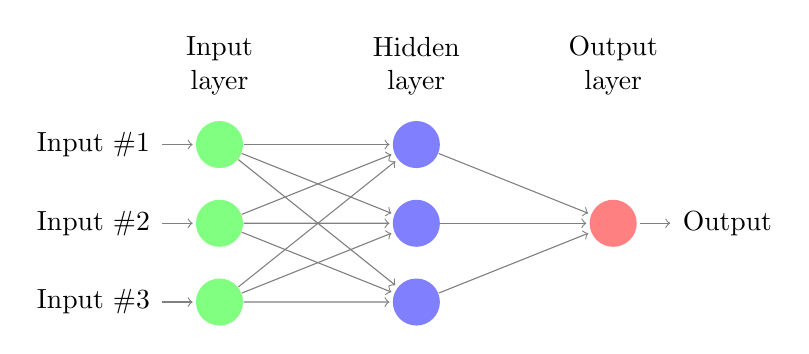
\begin{tikzpicture}[shorten >=1pt,->,draw=black!50, node distance=\layersep]
    \tikzstyle{every pin edge}=[<-,shorten <=1pt]
    \tikzstyle{neuron}=[circle,fill=black!25,minimum size=17pt,inner sep=0pt]
    \tikzstyle{input neuron}=[neuron, fill=green!50];
    \tikzstyle{output neuron}=[neuron, fill=red!50];
    \tikzstyle{hidden neuron}=[neuron, fill=blue!50];
    \tikzstyle{annot} = [text width=4em, text centered]

    % Draw the input layer nodes
    \foreach \name / \y in {1,...,3}
    % This is the same as writing \foreach \name / \y in {1/1,2/2,3/3,4/4}
        \node[input neuron, pin=left:Input \#\y] (I-\name) at (0,-\y) {};

    % Draw the hidden layer nodes
    \foreach \name / \y in {1,...,3}
        \path[yshift=0cm]
            node[hidden neuron] (H-\name) at (\layersep,-\y cm) {};

    % Draw the output layer node
    \node[output neuron,pin={[pin edge={->}]right:Output}, right of=H-2] (O) {};

    % Connect every node in the input layer with every node in the
    % hidden layer.
    \foreach \source in {1,...,3}
        \foreach \dest in {1,...,3}
            \path (I-\source) edge (H-\dest);

    % Connect every node in the hidden layer with the output layer
    \foreach \source in {1,...,3}
        \path (H-\source) edge (O);

    % Annotate the layers
    \node[annot,above of=H-1, node distance=1cm] (hl) {Hidden layer};
    \node[annot,left of=hl] {Input layer};
    \node[annot,right of=hl] {Output layer};
\end{tikzpicture}


Neural networks can be thought of a generalization of logistic regression where there is more than one layer of sigmoid transformations (activation functions). The activation units are denoted with the following notation:
\begin{align*}
& a_i^{(j)}: \text{activation of unit } i \text{ in layer } j \\
& \Theta^{(j)}: \text{Matrix of weights controlling function mapping from layer  } j \text{ to layer } j+1
\end{align*}

Specifically:
\begin{align*}
a_1^{(2)} &= g(z_1^{(2)}) = g \left( \Theta_{10}^{(1)}x_0 + \Theta_{11}^{(1)}x_1 + \Theta_{12}^{(1)}x_2 + \Theta_{13}^{(1)}x_3   \right)\\
%
a_2^{(2)} &= g(z_2^{(2)}) = g \left( \Theta_{20}^{(1)}x_0 + \Theta_{21}^{(1)}x_1 + \Theta_{22}^{(1)}x_2 + \Theta_{23}^{(1)}x_3   \right)\\
%
a_3^{(2)} &= g(z_3^{(2)}) =g \left( \Theta_{30}^{(1)}x_0 + \Theta_{31}^{(1)}x_1 + \Theta_{32}^{(1)}x_2 + \Theta_{33}^{(1)}x_3   \right)
%
\end{align*}

and:
\[
h(x) = a_1^{(3)} = g \left( \Theta_{10}^{(2)}a_0^{(2)} + \Theta_{11}^{(2)}a_1^{(2)} + \Theta_{12}^{(2)}a_2^{(2)} + \Theta_{13}^{(2)}a_3^{(2)}   \right)
\]

Each hidden layer gets an extra ``bias unit'' which inputs the constant value one: ($a_0^{(2)}$ = 1).

More compactly for a single training sample $(x,y)$:
\begin{align}
& a^{(1)} = x \quad \text{(add $x_0$)} \\
& z^{(2)} = \Theta^{(1)} a^{(1)} \\
& a^{(2)} = g(z^{(2)}\, ) \quad \text{(add $a_0^{(2)}$)} \\
& z^{(3)} = \Theta^{(2)} a^{(2)} \\
& a^{(3)}  = g(z^{(3)}\,) = h_\Theta (x)
\end{align}


 
To summarize, our hypothesis output is the logistic function applied to the sum of the values of our activation nodes, which have been multiplied by yet another parameter matrix $\Theta^{(2)}$ containing the weights for our second layer of nodes. Each layer gets its own wights matrix $\Theta$

The above computation can be vectorized for each layer from $j=2$ to $n$ where z, a, and $\Theta$ are matrices:
\begin{align*}
& z^{j} = \Theta\,^{j-1} \, {a^{\,j-1}}  \,  \\
& a^{\, j} = g(z^{j}) \quad \text{(add $a_0^{(j)}$)}
\end{align*}

%Or, fully vectorized:
%\[
%A = g(X \, \Theta)
%\]

The action of calculating the values of the hidden nodes, and finally the output nodes, based on the inputs is knows as forward propagation. 

A concrete example demonstrating how NNs work. The following implements an OR gate. Let $x \, \in \{0,1\}$ and $\Theta^{(1)} = [-10\quad 20\quad 20]$. Then: $h_\Theta(x) = g(-10 + 20x_1 + 20x_2)$. This will cause our hypothesis to be positive only if both $x_1$ and $x_2$ are $1$. (Recall that g is the sigmoid function, so is tends to 0 at $x=-4$ and to 1 at $x=+4$).
\begin{table}[htp]
\caption{default}
\begin{center}
\begin{tabular}{c c | c}
$x_1$ & $x_2$ & $h_\Theta(x)$\\
\hline
0 & 0 & $g(-10) \approx $ 0 \\
0 & 1 & $g(+10) \approx $ 1 \\
1 & 0 & $g(+10) \approx $ 1 \\
1 & 1 & $g(+30) \approx $ 1 
\end{tabular}
\end{center}
\label{default}
\end{table}%

Alternative, by setting the intercept to -30 one can implement an AND gate:
\[
\Theta^{(1)} =  [-30\quad 20\quad 20]
\]
Or a NOR gate:
\[
\Theta^{(1)} =  [10\quad -20\quad -20]
\]
By combining the X1 AND X2 gate, and the NOR gate ((NOT X1) AND (NOT X2)) gate as a hidden unit, and X1 OR X2 gate as output unit, we can build a XNOR gate:
\[
\begin{bmatrix}
x_0\\x_1\\x_2
\end{bmatrix}
\rightarrow
\begin{bmatrix}
a_0\\a_1^{(2)}\\a_2^{(2)}
\end{bmatrix}
\rightarrow
\begin{bmatrix}
a^{(3)}\\
\end{bmatrix}
\rightarrow h_\Theta(x)
\]

So:
\begin{align*}
&a^{(2)} = g(\Theta^{(1)}\, x)\\
&a^{(3)} = g(\Theta^{(2)}\, a^{(2)}) \\
&h_\Theta(x) = a^{(3)}
\end{align*}

For multi-class classification we set the output layer to be a number of nodes, instead of a single node, so that the NN outputs vectors. Accordingly, we change the labels from scalers to vectors. So if an image can be one of four things then the label representing thing four takes the form of:
\[
y^{(i)} = 
\begin{bmatrix}
0\\0\\0\\1
\end{bmatrix}
\]

\paragraph{Training NNs:}
The first step is forward propagation and calculation of a cost. The cost function is as follows. If  the output for each observation is a vector $h_\Theta \in \mathbb{R}^K$, and $h_\Theta(x^{(i)})_k$ is the $k^\text{th}$ entry of the output, then the cost function is similar to the cost for logistic regression but summed over all k entries of the output vector of each sample, as well as over all samples:
\[
J(\Theta) = -\frac{1}{m} \left[ \, \sum_{i=1}^m	 \sum_{j=1}^K  \,
	y_k^{(i)} \log h_\Theta (x^{(i)})_k +
	(1 - y_k^{(i)}) \log \left( 1 - h_\Theta (x^{(i)})_k \right)
	\right] + \text{R}
\]
The regularization term R is similar to the regularization term for logistic regression, but now every entry of every matrix $\Theta^{(l)}$ is squared and the whole lot is summed together across all rows, all columns, and all matrices:
\[
R = \frac{\lambda}{2m} \sum_{l=1}^{L-1} \sum_{i=1}^{s_l} \sum_{j=1}^{s_{l+1}} (\Theta_{ji}^{(l)} )^2
\]
Here $L$ is the total number of layers in the network and $s_l$ is the number of units (not including bias) in layer $L$. 

Alternatively, define a matrix Y such that:
\[
Y = 
\begin{bmatrix}
{ --- \left( y^{(1)} \right)^T --- }\\[0.5em]
{ --- \left( y^{(2)} \right)^T --- }\\
\end{bmatrix}
\]

and similarly define a matrix H which consists of all the hypotheses $h_\Theta(X)$ for all samples
\[
H = 
\begin{bmatrix}
{ --- \left( h_\Theta (x^{(1)}) \right)^T --- }\\[0.5em]
{ --- \left( h_\Theta (x^{(2)}) \right)^T --- }\\
\end{bmatrix}
\]
then:
\[
J(\Theta) = 
-\frac{1}{m}\Big[ \sum_{column} \sum_{rows} \big( Y \otimes \log H + (1-Y) \otimes \log(1-H) \big) \Big] + R
\]
where $\otimes$ denotes element-wise multiplication and R is:
\[
R  = \frac{\lambda}{2m} \left( \, \sum_{column} \sum_{rows} L \Theta_1^{\otimes2}  + \sum_{column} \sum_{rows} L \Theta_2^{\otimes2}  + \dots \right)
\]
where $L$ chooses all columns but the first one (we don't regularize the bias wieghts), and the squaring is performed element-wise. 

The next step is back-propagation and calculation of gradients of the cost with respect to the various parameters. The intuition here is that $\delta^{(l)}_j$ is the ``error'' of node $j$ in layer $l$.

Example for a four-layer NN:
\begin{align*}
&\delta^{(4)} = a^{(4)} - y \\
&\delta^{(3)} = (\Theta^{(3)})^T \, \delta^{(4)} \otimes g^{\prime} (z^{(3)})	\\
&\delta^{(2)} = (\Theta^{(2)})^T \, \delta^{(3)} \otimes g^{\prime} (z^{(2)})	
\end{align*}
where $g^{\prime}(z^{(l)}) = a^{(l)} \otimes (1 - a^{(l)})$. There is no $\delta^{(1)}$. The values of $\delta$ can then be used to calculate the derivatives:
\[
\frac{\partial}{\partial \Theta_{ij}^{(l)}}J(\Theta) =
a_j^{(l)}\delta_{i}^{(l+1)}
\]

The backprop algorithm is as follows:


\newpage{}

\section{Resampling Methods}
%All human things are subject to decay. And when fate summons, Monarchs must obey.
%]
\begin{itemize}
\item k-fold cross validation: 
\[
\text{CV}_{(k)} =
\frac{1}{k} \sum^k_{i=1}\text{MSE}_i
\]
\item LOOCV is simply a special case of k-fold CV where k=n.
\item With linear least-squares models the following holds:
\[
\text{CV}_{(n)} = \frac{1}{n}\sum^n_{i=1}
\left( \frac{y_i - \hat y_i}{1 - h_i} \right)^2
\]
where $y_i$ is the $i$th value from the original least squares fit and $h_i$ is the leverage (for linear regression):
\[
h_i = \frac{1}{n} + \frac{(x_i - \bar x)^2}
{
\sum^n_{i'=1}(x_{i'}-\bar x)^2 
}
\]
\item In a classification setting we use the number of missclassified observations:
\[
\text{CV}_{(n)}=\frac{1}{n}
\sum^n_{i=1}Err_i
\]

\end{itemize}


\section{Tree-Based Methods}



For classification trees the deviance (as reported in  \texttt{summary}):
\[
d = -2 \sum_m \sum_k n_{mk} \log \hat{p}_{mk}
\]

where $n_{mk}$ is the number of observations in the $m$th terminal node that belongs to the $k$th class. The residual mean deviance is the deviance divided by $n-|T_0|$ where n is the number of observation and $T_0$ is the number of terminal nodes. Here $\hat p_{mk}$ represents the proportion of training observations in the $m$th
region that are from the $k$th class.

The residual mean deviance is reported by dividing the deviance by $n - T_0$, where $T_0$ is the terminal number of nodes. 
\[
RMD = \frac{d}{n-|T_0|}
\]

\section{Hashing Trick}

A hash table is a dictionary. It uses a hash function to map keys to indices of buckets which contain values. Many hash tables have imperfect hashing  in which different keys have the same index in the table (collisions). On the other hand, hash tables have efficient lookup: the average cost is independent of the number of elements stored in the table. In many situations hash able turn out to be more efficient than search trees or other table lookup structures.  

\section{Metrics}

\paragraph{Confusion matrix: } True on the rows and predicted on the columns.

\begin{table}[h]
\centering
\begin{tabular}{ll|l|l|}
\cline{3-4}
                                            &   & \multicolumn{2}{l|}{Predicted} \\ \cline{3-4} 
                                            &   & T              & F             \\ \hline
\multicolumn{1}{|l|}{\multirow{2}{*}{TRUE}} & T & TP             & FN            \\ \cline{2-4} 
\multicolumn{1}{|l|}{}                      & F & FP             & TN            \\ \hline
\end{tabular}
\end{table}



\paragraph{Precision: } aka positive predictive value (PVV). Is correctly identified positives over all predicted positives.
\[
\mathrm{Precision} = \frac{\mathrm{TP}}{\mathrm{ TP+FP}}
\]

\paragraph{Recall: }
aka sensitivity, true-positive rate (TPR). Is the correctly identified positives over all actual positives.
\[
\mathrm{Recall} = \mathrm{\frac{TP}{TP+FN}}
\]

\paragraph{P-R curve} As recall is a measure of false negatives and precision is a measure of false positives there is a tradeoff between them. One could capture all terrorists (reduce false negatives) by accusing the entire population of being terrorists. One could try to reduce false positives (false accusations) by accusing only a small number of people. This would naturally result in a few getting through (false negatives). If one starts with a low threshold (accusing everybody) and slowly increases it then one moves from high recall to high precision. Ideally even at a low threshold one has high precision. Hence the area under the P-R curve can serve as a metric. 


\paragraph{Fallout} aka false-positive rate (FPR), is the ratio of false-positives (incorrectly identified negative) to actual negatives (both correctly and incorrectly identified). Gives probability of a false alarm.
\[
\text{Fallout} = \mathrm{\frac{FP}{FP+TN}}
\]

\paragraph{ROC curve} It is a plot of the recall  (sensitivity, TPR) against fallout (FPR) for the different possible thresholds of a diagnostic test (T). 


\paragraph{}





\paragraph{Accuracy: } Fraction of instances where predicted score equals actual score. 
\[
\text{accuracy} = \mathrm{\frac{TP + TN}{TP+TN+FP+FN}}
\]
Calculated with:
\[
\mathrm{accuracy(y,\hat y)} = \frac{1}{n_{samples}} \sum_{i=0}^{n-1} 1_{\hat y_i = y_i}
\]



\paragraph{F1-score:}
\[
\mathrm{F_1\text{-score}} = \mathrm{2 \frac{precision \cdot recall}{precision + recall}}
\]






\section{Combinatorial Analysis}

\paragraph{The basic principle of counting:} If there are two experiments, one with n outcomes and one with m outcomes, then there are $m\,n$ possible outcomes of the two experiments. More generally, if there are $r$ experiments each with $n_i$ outcomes, then the total number of outcomes is $n_1\cdot n_2 \cdot n_3 \dots = \prod_{i = 1}^n n_i$

\paragraph{Permutations:} How many permutations of the letters $a\,b\,c$ are there? First option is for either one of the three, then the remaining two, and then the remaining one. So in total $2\cdot 2\cdot 1 = 6$. In general, if there are $n$ different items to permute, then there are $n\cdot (n-1)\cdot \dots \cdot 2 \cdot 1 = n!$ options.

\paragraph{Permutation of identical objects:} How many arrangements of the letters PEPPER are there? There are 6!\ possible arrangements of the letters but there are 3!\ identical permutations of P and 2!\ identical permutations of E. So in total there are $\frac{6!}{3!\,2!}$ unique permutations. In general, given n objects, of which n$_1$ are alike, n2 are alike and so forth, then there are 
\[
\frac{n!}{n_1! \, n_2! \dots n_r!}
\]

\paragraph{Combinations:} How many different groups of 3 can be formed from the letters ABCDE? There are 5 ways to choose the first member of the group, 4 of the second, and 3 of the third, so $5\cdot4\cdot3 = \frac{5!}{2!}$ possible permutations of groups of three, but within group permutations (BAC, CBA \dots) do not count so need to divide by $3!$. In total $\frac{5!}{(5-3)!\,3!} = 10$ groups can be formed. In general, there are such many ways to form r groups out of n objects:
\[
{{n}\choose{r}} = \frac{n!}{(n-r)! \, r!}
\]
%
This represents the number of different groups of size r that could be selected from a set of n objects when the order of selection is not considered relevant.

%The following identity can sometimes by helpful:
%\[
%{{n}\choose{r}} = {{n-1}\choose{r-1}} + {{n-1}\choose{r}}
%\]

\paragraph{Binomial Coefficients:} 
The values ${n}\choose{k}$ are sometimes known as binomial coefficients since they play a role in the binomial theorem:
\[
(x+y)^n = \sum^n_{k = 0} {{n}\choose{r}} x^k \, y^{n-k}
\]

\paragraph{Multinomial coefficients:} A set of $n$ distinct objects is to be divided into $r$ groups of varying sizes $n_1, n_2, \dots, n_r$ that sum up to $n$. How many possible partitions are there? 
\[
{{n}\choose{n_1, n_2, \dots, n_r}} = \frac{n!}{n_1!\,n_2!\dots n_r!}
\]

The multinomial coefficients show up in the generalization to the binomial theorem, which is known as the multinomial theorem:
\[
(x_1 + x_2 + \dots + x_r)^n = \sum {{n}\choose{n_1,n_2,\dots,n_r}} x^{n_1} \, {x_2}^{n_2} \dots {x_r}^{n_r}
\]

\paragraph{Summation permutations:} A group of $n$ objects is to be decomposed into $r$ non-negative groups of unknown sizes. How many possible partitions are there?
\[
{n+r-1}\choose{r-1}
\]

\section{Conditional Probability}

\paragraph{Conditional Probability}

\[
P(E|F) = \frac{P(E \cap F)}{P(F)}
\]

\paragraph{The Multiplication Rule}
\[
P(E_1\,E_2\,\dots\, E_n) = P(E_1)\,P(E_2|E_1)\,P(E_3|E_1\,E_2)\dots \,P(E_n|E_1\,E_2 \dots E_{n-1})
\]


\paragraph{Bayes's Formula}
Conditional times marginal equals conditional times marginal equals joint. Useful for evaluating conditional probabilities. 
\begin{align*}
P(F|E)\,P(E)= P(EF) = P(E|F)\,P(F)  
\end{align*}
%
\begin{align*}
P(F|E) = \frac{ P(E|F)\,P(F) }{P(E)}
\end{align*}
%
\begin{align*}
P(E) &= P(EF) + P(EF^c) \\
     &= P(E|F)\,P(F) + P(E|F^c)\,P(F^c) \\
     &= P(E|F)\,P(F) + P(E|F^c)[1-P(F)]
\end{align*}

\paragraph{Odds of an event}
The odds of an event happening are defined as:
\[
\frac{P(E)}{P(E^c} = \frac{P(E)}{1-P(E)}
\]


Thus, if hypothesis $H$ is true with probability $P(H)$, how do the odds of the hypothesis change with the introduction of new evidence E?
\begin{align*}
\frac{P(H|E)}{P(H^c|E)} = \frac{P(H)}{P(H^c)} \frac{P(E|H)}{P(E|H^c)}
\end{align*}
%
The new odds of the hypothesis being correct are the old odds weighted by the odds of the the likelihood of the evidence given the correctness of the hypothesis. 


\paragraph{Bayes's formula for multiple events}
\[
P(F_j|E) = \frac{P(E\,F_j)}{P(E)} = \frac{P(E|F_j)\,P(F_j)}{\sum^n_{i=1} P(E_i|F_i)\,P(F_i) }
\]

\paragraph{Independent Events} If E and F are independent then:
\[
P(EF) = P(E)\,P(F)
\]








\end{document}  

















